% Data,
% Data set,
% Source,
% Preprocecing,
% Data visualization


\section{MNIST}

MNIST data contains 70,000 samples of handwritten labeled digits \cite{1} 

\subsection{Pre-processing}

MNIST images have fixed dimensions (28 X 28 X 1), and therefore the only preprocessing is normalizing the range of pixels values from [0, 255] to [-1, 1].



\subsection{Visualisation}

\begin{figure}[h]
\centering
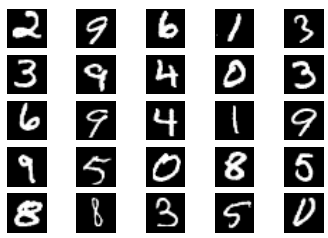
\includegraphics[scale=0.8]{MNIST-sample}
\caption{MNIST random sample}
\label{fig:x cubed graph}
The digits variate in style - we can see different widths, orientations and curvatures for every image.
\end{figure}


\section{IAM}

IAM data contains approximately 115,000 images of label handwritten words.  \cite{2} 

\subsection{Pre-processing}

Words images were re-sized to the size of (16n, 32), where n is the length of the word (number of letters in the label). The idea here is to artificially make each character have an approximate dimensions of (16, 32) in the generated image. 
Outliers (images with much longer or shorter width of 16n) were removed, as they are not the typical handwriting that we want to examine in the scope of this project.
Also, as stated before, the pixels values was normalized to a range of [-1, 1]. 


\subsection{Visualisation}

\begin{figure}[h]
\centering
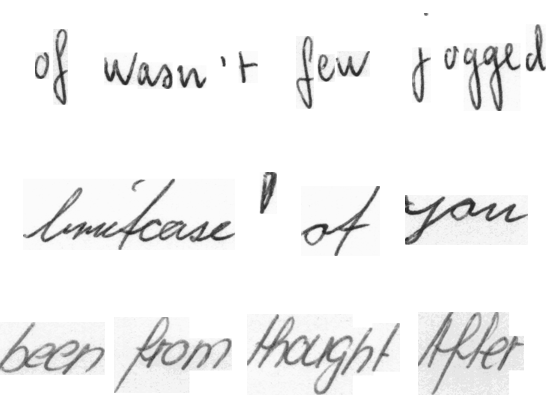
\includegraphics[scale=0.8]{IAM-sample}
\caption{IAM random sample}
\label{fig:x cubed graph}
Each row is a sample from a different writer. Notice the inter-group variance vs the intra-group variance - the way the style differs from one writer to another, and the difference between the same letters by the same writer. We want to capture both of these variances in our modeling process.
\end{figure}